\chapter{Implementation}

% Containing a comprehensive description of the implementation of your software, including the language(s) and platform chosen, problems encountered, any changes made to the design as a result of the implementation, etc.

Agile development processes have been followed throughout the entirety of the project, with the key indicator of progress being working code. As a result, a significant amount of implementation has taken place, with the implementation in its current state being close to a Minimal Viable Product; although there are some key features that have not yet been implemented.

\section{Languages and Tools}

Some of the technical decisions regarding language choice are limited by virtue of the architectural decision to build the application using Electron. As a result the primary programming language for the project will be JavaScript. Being able to use JavaScript for both the frontend user interface and the backend service means less context-switching and a more rapid development process. To aid in rapid development of a user interface, a Frontend JavaScript framework will be used. The three primary candidates for the framework choice were React, Vue and Angular. Since I have prior experience with React, and felt that the rate of work would benefit from not having to learn a new framework, React was chosen as the frontend framework for this project.

Alongside JavaScript, Electron and React, there are a number of other tools being utilised to aid development. Babel and Webpack are being used to transpile and bundle JavaScript modules, respectively. 

\section{Testing}

In order to ensure that software is of a high quality, significant testing must be carried out. The project will be tested by means of Unit Tests, Functional (End-to-End) tests, and User Acceptance Tests (UAT).

\subsection{Unit Testing}
During the development process so far, unit tests have been written alongside the source code. The tests have been written using the Open Source test framework, Jest. The primary reason why Jest was chosen as the testing framework for this project was due to its Snapshot Testing feature \cite{jest-snapshot}, allowing tests to take a snapshot of a React component's output and then compare all future test runs to this snapshot. This leads to much cleaner test code, which can be written more quickly. In addition, the tests for React components use the Enzyme library for manipulating, traversing, and simulating interaction events on the component output \cite{enzyme}. The full unit test suite is run before feature branches can be merged into the master branch, as regression testing to ensure that new functionality does not cause other tests to fail. A soft target of a minimum of 90\% unit test coverage has been set to increase the likelihood of the tests reliably identifying problems. The master branch currently has unit test coverage of 98.41\%, and a full coverage report can be found in Appendix \ref{appendix:coverage}.

\subsection{Functional Testing}
In addition to the unit tests described previously, this project will make use of automated Functional (End-to-End) tests in order to ensure that the functional requirements of the system are met. The functional tests will be based on the Functional Specification for this project, as outlined in Section \ref{sec:functional-spec}. Initially, a functional test runner, Spectron, was set up in the project; however, at present there are problems with the test runner, and work is ongoing to identify and resolve the issue.

\section{Electron Application Architecture}
As discussed previously the application is being built using the Open Source JavaScript Framework, Electron. Electron has two different types of process; the main process, and renderer processes \cite{electron-architecture}. Each renderer process has the ability to optionally display a web page inside a \textit{BrowserWindow}. 

The initial architectural implementation of the application had two processes: the main process and a single renderer process. The main process is the parent process to all of the renderer processes, and it is the only process that is able to call native GUI APIs \cite{electron-architecture}. This original idea would use the renderer process for displaying the React user interface, and the main process for running the email client services. By keeping the long-running service in a separate process, the performance of the React app would not be hindered. However, further research indicated that this architecture would not be suitable.

The main process houses the UI thread, and therefore it is imperative that it is not blocked with long-running operations to avoid the whole application from freezing until the main process becomes available again \cite{electron-performance}. As a result, the application was re-architected to make use of two renderer processes; one for the react app and one for the email service, in addition to the main process. These two renderer processes are able to communicate with each other using Electron's built in Inter-Process Communication (IPC) methods. Initially, the two renderer processes are unable to directly communicate with each other, and so the main process must first use IPC to send each of the renderer processes the ID of the other, which they can then use for direct message passing. The nature of this communication initialisation is shown by figure \ref{fig:sequence-ipc}.

\begin{figure}[h!]
\begin{center}
  \begin{tikzpicture}
    \coordinate (a) at (0,0);
    \coordinate (b) at (0,6);
    \coordinate (c) at (5,0);
    \coordinate (d) at (5,6);
    \coordinate (e) at (10,0);
    \coordinate (f) at (10,6);
    \draw [dashed] (a) -- (b)node[pos=1.1,scale=1]{Service Renderer} (c) -- (d)node[pos=1.1,scale=1]{Main}
    (e) -- (f)node[pos=1.1,scale=1]{UI Renderer};
    \draw[{Latex[length=3mm]}-] ($(a)!0.90!(b)$) -- node[below,scale=1,midway]{broadcast-ui-id}($(c)!0.90!(d)$);

    \draw[-{Latex[length=3mm]}] ($(c)!0.70!(d)$) -- node[below,scale=1,midway]{broadcast-service-id}($(e)!0.70!(f)$);

    \draw[{Latex[length=3mm]}-] ($(a)!0.50!(b)$) -- node[below,scale=1,midway]{submit-login-info} ($(e)!0.50!(f)$);

    \draw[-{Latex[length=3mm]}] ($(a)!0.30!(b)$) -- node[below,scale=1,midway]{login-success} ($(e)!0.30!(f)$);

    \draw[-{Latex[length=3mm]}] ($(a)!0.10!(b)$) -- node[below,scale=1,midway]{login-failure} ($(e)!0.10!(f)$);

  \end{tikzpicture}
  \caption{Sequence Diagram showing nature of IPC between Electron processes}
  \label{fig:sequence-ipc}
\end{center}
\end{figure}

\section{Email Sending and Receiving Prototype}
\subsection{Sending}

\subsection{Receiving}

\section{User Interface}
\begin{figure}[h!]
  \centering
  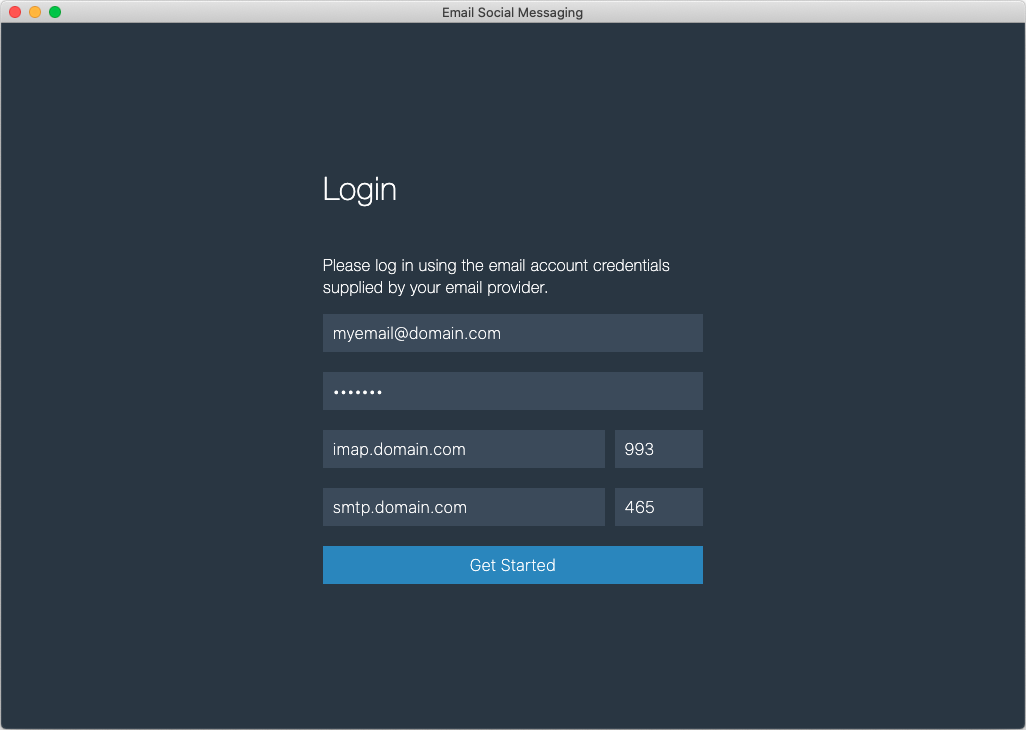
\includegraphics[width=\textwidth]{images/implementation-login.png}
  \caption{Initial Design}
\end{figure}

\begin{figure}[h!]
  \centering
  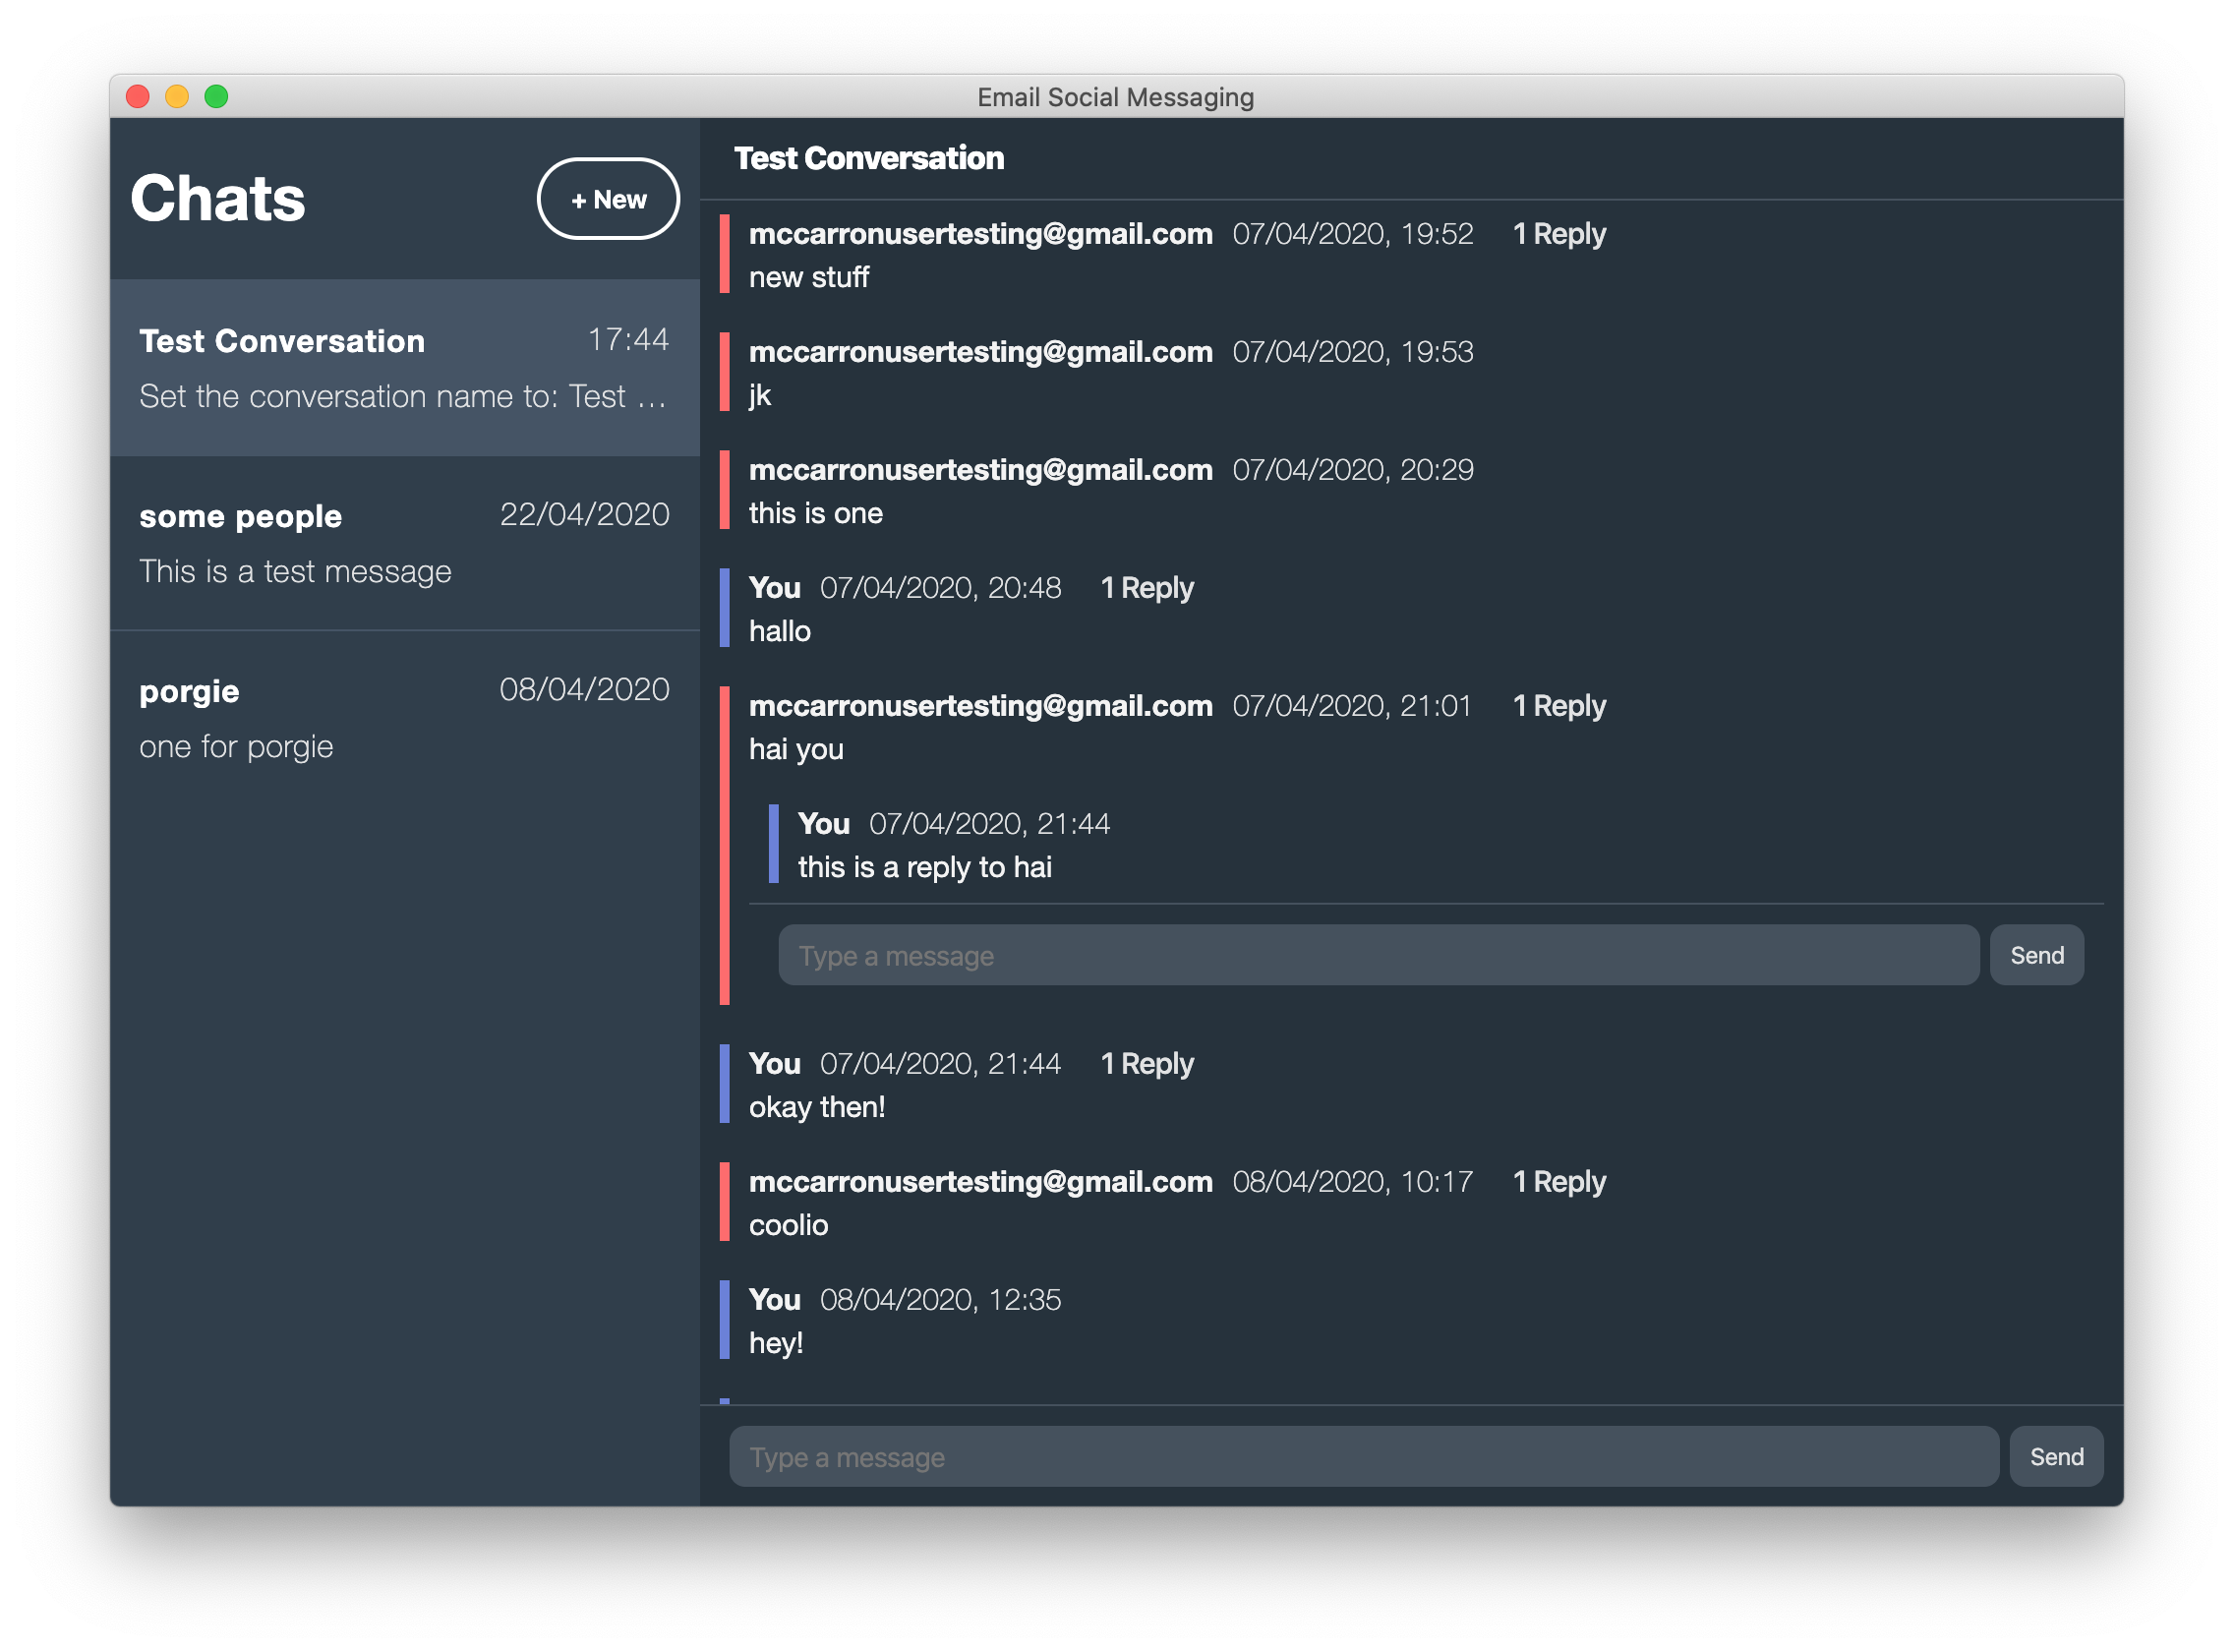
\includegraphics[width=\textwidth]{images/implementation-main.png}
  \caption{Initial Design}
\end{figure}